\section{Previous curses resume}
\subsection{Internal loads}
	For the internal loads the following differential equations can be considered:
	\[ \frac{dM_z}{dz} + m_z(z) = 0 \qquad \frac{dM_x}{dz} -T_y(z) + m_x(z) = 0 \qquad \frac{dM_y}{dz}  + T_x(z) + m_y(z) = 0  \]

\subsection{Stress distribution}
\begin{multicols}2
\subsubsection{Axial load}
	Given the normal load $N$ on a beam having area $A$ then the stress distribution is constant and
	\[\szz = \frac N A \qquad \Rightarrow \quad \ezz = \frac{N}{EA}\]
	The elastic potential energy related to such action is
	\[dU_e = \frac{N^2}{2EA} dz\]
\subsubsection{Bending moments}
	The stress  state of a shaft subjected to bending moments $M_x,M_y$ depends on the position and the moments of inertia $I_x,Y_y$ referred to the barycentric system, and so
	\[ \szz = \frac{M_x}{I_x} y - \frac{M_y}{I_y}x \qquad \Rightarrow \quad \ezz = \frac{M_x} {EI_x} y - \frac{M_y}{EI_y}x \]
	and the elastic potential energy is
	\[ dU_e = \left( \frac{M_x^2}{2EI_x} + \frac{M_y^2}{2E I_y} \right)dz \]
	
\subsubsection{Torsion moment}
	The torsional elastic potential energy is
	\[ dU_e = \frac{M_z^2}{2GJ_p} dz \qquad \textrm{where } G = \frac{E}{2(1+\nu)} \]	
	and the torsional module $J_p$ is
	\begin{align*}
		J_p & = \int_A \left( x^2 + y^2 + x \frac{\partial \psi}{\partial y} - y \frac{\partial \psi}{\partial x} \right) dA \\ & = I_x + I_y + \int_A \left(	 x \frac{\partial \psi}{\partial y} - y \frac{\partial \psi}{\partial x} \right) dA
	\end{align*}
	
	\paragraph{Circular section} For a circular section the shear component evaluates as
	\[ \tlz = G \theta r = \frac{M_z}{J_p} r \]
	
	\paragraph{Thin section} For section with thin walls it's possible to use the Breadt formula that says
	\[ \tlz = \frac{M_z}{2s\Omega} \]
	where $s$ is the thickness of the wall and $\Omega$ is the area of the section referred to the mean wall line.
	
\subsubsection{Shear action}	
	In general shear action can be neglected when $L/b>10$ ($L$ length of the beam, $b$ dimension of the section). In the case it's necessary to compute such values we can use Jourawsky theory for which
	\[ \qquad \tau_x (x) = \frac{V_x S_y^*(x)}{I_y b(x)} \qquad \tau_y (y) = \frac{V_y S_x^*(y)}{I_x b(y)} \]
	
\end{multicols}
	
\subsection{Properties of the section}
	\paragraph{Rectangle} Given a rectangle with base $b$ (dimension over $x$ axes) and height $h$, then the section's geometry are $A=bh$, $I_x = \frac{bh^3}{12}$ and $I_y = \frac{b^3h}{12}$. 
	\begin{multicols}{2}
		If the section is hollow as in the adjacent figure then the parameters are
		\begin{align*}
			 A & = bh  - (h-2s_1)(b-2s_2)  \\
			 I_x & = \frac{bh^3}{12} - \frac{(b-2s_2)(h-2s_1)^3}{12}\\
			 I_y & = \frac{b^3h}{12} - \frac{(b-2s_2)^3(h-2s_1)}{12} 
		\end{align*}
		In both cases $J_p = I_x + I_y$.
		\begin{center}
			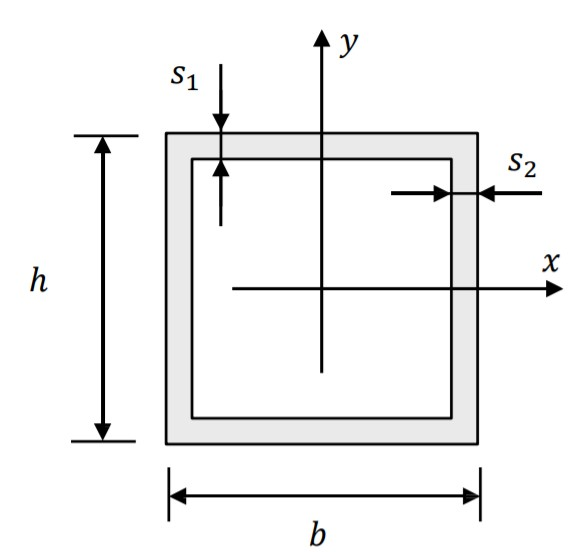
\includegraphics[width=5cm]{hollow-rect}
		\end{center}
	\end{multicols}
	
	\paragraph{Circle} A circular section of diameter $D$ has $D = \frac \pi 4 D^2$, $I_x = I_y = \frac \pi {64}D^4$ and $J_p = I_x + I_y = \frac \pi {32} D^4$; if the section is hollow with external and internal diameters $D_e,D_i$, then
	\[ A = \frac\pi 4 \big(D_e^2-D_i^2\big) \qquad \qquad I_x = I_y = \frac \pi {64}\big(D_e^4-D_i^4\big) \qquad \qquad J_p = \frac \pi {32} \big(D_e^4-D_i^4\big) \]
	

	\paragraph{H section} Given the H(I) section (figure \ref{fig:THsections}.a) then the area is computed as $A = bh - (b-a)(h-2e)$ with moment of inertia 
	\[ I_x = \frac{bh^3}{12}- \frac{(b-a)(h-2e)^3}{12} \qquad \qquad I_y = \frac{b^3e}{6} + \frac{a^3(h-2e)}{12} \]
	and polar moment of inertia $J_p = I_x + I_y$.
	
	\begin{figure}[bht]
		\centering
		\begin{subfigure}{0.48\linewidth}
			\centering 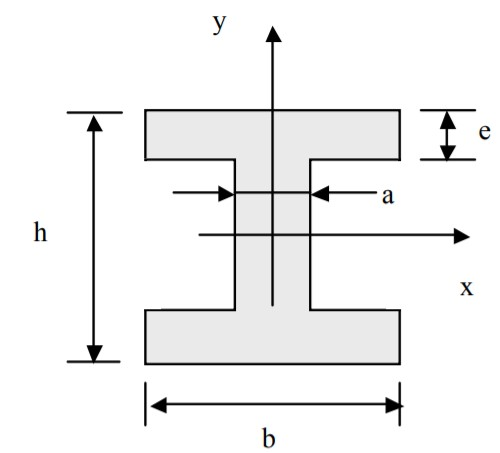
\includegraphics[width=5cm]{H-section} \caption{}
		\end{subfigure}
		\begin{subfigure}{0.48\linewidth}
			\centering 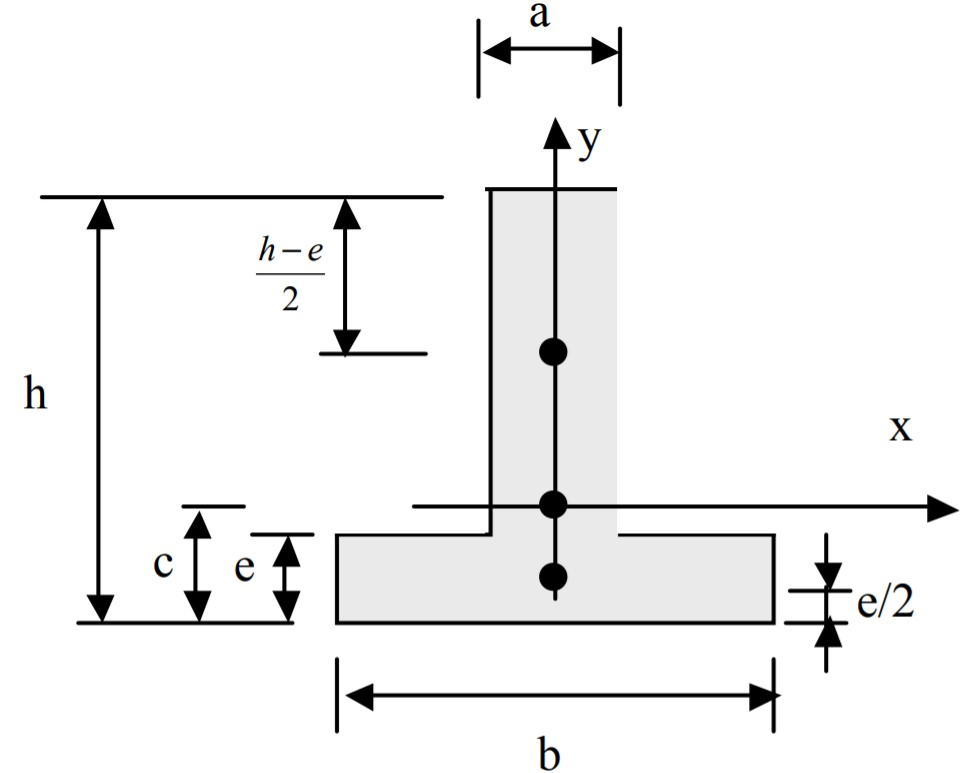
\includegraphics[width=6cm]{T-section} \caption{}
		\end{subfigure}
		\caption{schematic representation of the $H$ section (a) and the $T$ one (b).} \label{fig:THsections}
	\end{figure}
	
	\paragraph{T section} Given the T section in figure \ref{fig:THsections}.b, the area is $A = be + a(h-e)$ and the centroid of the area (where the principal axis are positioned) is computed as
	\[ c = \frac 1 2 \frac{be^2 + a(h^2-e^2)}{be + a (h-e)} \]
	The moments of inertia respect the barycentric axis are
	\[ I_x = \frac{be^3}{12} + be\left( c-\frac e2\right)^2 + \frac{a(h-e)^3}{12} + \frac{a(h-e)\left( \frac{h-e}{2} - c \right)}{2} \qquad \qquad I_y = \frac{be^3}{12} + \frac{a^3(h-e)}{12} \]
	The polar moment of inertia is $J_p = I_x + I_y$.
	
	
	
	
	
	
	
	
	
	
	
	
	
	
	
	
	
	
	
	
	
	
	
		